\section*{Introduction}
\chead{Introduction}
\addcontentsline{toc}{section}{Introduction}

Bioinformatics is an interdisciplinary field that applies computational
methods to the analysis, organization, and interpretation of biological data.
Its primary objective is to extract meaningful biological insights from large
and often heterogeneous datasets, such as genomic sequences, transcriptomic
measurements, and protein structures. With the advent of high-throughput
experimental technologies, bioinformatics has become an essential component of
modern biological research, enabling analyses that would be prohibitively
time-consuming and expensive through purely experimental approaches.

A central object of study in bioinformatics is the biological sequence. In the
context of molecular biology, a biological sequence refers to an ordered string
of symbols representing nucleotides (DNA or RNA) or amino acids (proteins).
Protein sequences, in particular, play a crucial role in understanding cellular
function, as the structure and activity of proteins directly shape most
biological processes. Given the large number of proteins encoded in a genome and
their diverse functional roles, comprehensive analysis at scale is required to
systematically characterize their properties. Consequently, the large-scale
analysis of protein sequences has become a foundational task in computational
biology.

\subsection*{Motivation and Scale of the Problem}

Public biological databases have grown at an unprecedented rate over the past
two decades. Advances in \textit{Next-generation Sequencing} (NGS) technologies
have enabled the rapid and cost-effective determination of DNA and RNA
sequences from biological samples at massive scale. As a result, repositories
such as Universal Protein Resource (UniProt) \cite{uniprot} now contain
billions of nucleotide sequences and hundreds of millions of protein sequences,
with new data added continuously. In particular, the size of microbial sequence
databases, has outpaced the capabilities of traditional alignment tools
\cite{lexicmap}. While sequence generation has become increasingly efficient,
the downstream analysis of these data has emerged as a major computational
bottleneck.

One fundamental analytical task is sequence clustering: the grouping of
biological sequences based on similarity. Sequence clustering is widely used to
identify protein families, infer evolutionary relationships, reduce redundancy
in large datasets, and support downstream analyses such as functional
annotation and structural prediction. In practical applications, clustering
serves as a data reduction mechanism, allowing researchers to operate on
representative groups rather than on individual sequences.

The importance of sequence clustering is further highlighted by the high cost
and complexity of experimentally determining protein structures. Experimental
protein structure determination has historically relied on X-ray
crystallography, NMR spectroscopy, and cryo-electron microscopy. While these
methods produce high-quality structures, they are slow and costly, requiring
specialized facilities and extensive human effort. Prior to recent
computational advances, the global collection of experimentally determined
protein structures comprised on the order of 100,000 unique entries,
accumulated over several decades. Estimates suggest that assembling such a
dataset required international collaboration spanning more than forty years and
financial investments on the order of several billion U.S. dollars, with
per-structure costs ranging from 50,000 to 100,000 \cite{PNNL13501}.

\subsection*{Problem Formalism \& Community Detection}

Community detection is a class of algorithms aimed at identifying groups of
nodes in a graph that are more densely connected to each other than to the rest
of the graph. In the context of \textit{Protein Sequence Similarity Networks}
(PSSNs), these communities can be interpreted as clusters of related sequences.
Sequence similarity networks offer a scalable and interpretable representation
of relationships, accommodating far larger datasets than traditional
phylogenetic trees or multiple sequence alignments \cite{ssn}. Among the many
community detection algorithms proposed in the literature, the Markov
Clustering Algorithm (MCL) \cite{mcl} has been widely adopted in bioinformatics
due to its robustness and ability to capture complex cluster structures.

The standard MCL algorithm is limited in scalability by its memory requirements
and computational complexity, particularly during matrix expansion steps.
A high performance variant called HipMCL \cite{hipmcl}, can leverage multiple
processes and distributed sparse matrix operations for very large graphs. In
this work, however, all experiments are conducted on a single compute node.
Accordingly, HipMCL is executed in single-node mode, with parameters chosen to
ensure efficient memory usage and reproducible results.

\subsection*{Motivation \& Problem Scale}

Recent breakthroughs in computational biology, most notably the development of
AlphaFold \cite{alphafold}, have ushered in a new era where large-scale
computation and machine learning are rapidly transforming molecular biology.
In recognition of its impact on protein structure prediction, Demis Hassabis
and John Jumper were each awarded half of the 2024 Nobel Prize in Chemistry for
the development of AlphaFold, with the other half awarded to David Baker for
contributions to computational protein design. AlphaFold's ability to predict
protein structures with high structural precision has significantly expanded the
availability of structural data, effectively addressing a long-standing
challenge in molecular biology. However, even with such advances, many
computational pipelines continue to rely on intermediate preprocessing steps
that operate directly on large collections of protein sequences, such as
similarity search, protein graph construction, and its subsequent partitioning
into communities.

With the latest advances in high-throughput sequencing, protein sequence
datasets analyzed in large-scale studies often span tens of millions to
billions of sequences. The scale and structural heterogeneity of such data 
and the computational demands they often impose are illustrated in
Fig.~\ref{fig:darkMatter}, showing the work performed in \cite{darkMatter},
clustering over 1.7 billion protein sequences using HipMCL on approximately
2,500 compute nodes, starting from over 100,000 reference genomes and 26,000
metagenomes. Similarity filtering produced graphs with hundreds of millions of
nodes and billions of edges --- extremely sparse (density below \(10^{-7}\))
yet massive in absolute size. 

This raises a practical question:
\begin{center}
  How far can HipMCL and standard MCL scale on a single compute node?
\end{center}
The present study addresses this gap by systematically
evaluating both algorithms on a single compute node using datasets up to 82
million sequences.
% Logic: Large‑scale distributed clusters with thousands of nodes are expensive and not available to most academic research groups. Therefore, understanding what can be achieved on a single node --- which is the common academic setting --- is practically relevant.

Furthermore, in Fig.~\ref{fig:darkMatter}~(b), metagenomes exhibit superlinear
growth, indicating that newly added datasets contribute disproportionately many
novel protein families. Hence, it makes more sense to limit our investigation
on reference genomes which are computationally more stable and predictable in
sequence alignment and clustering.

\begin{figure}[htbp]
  \centering
  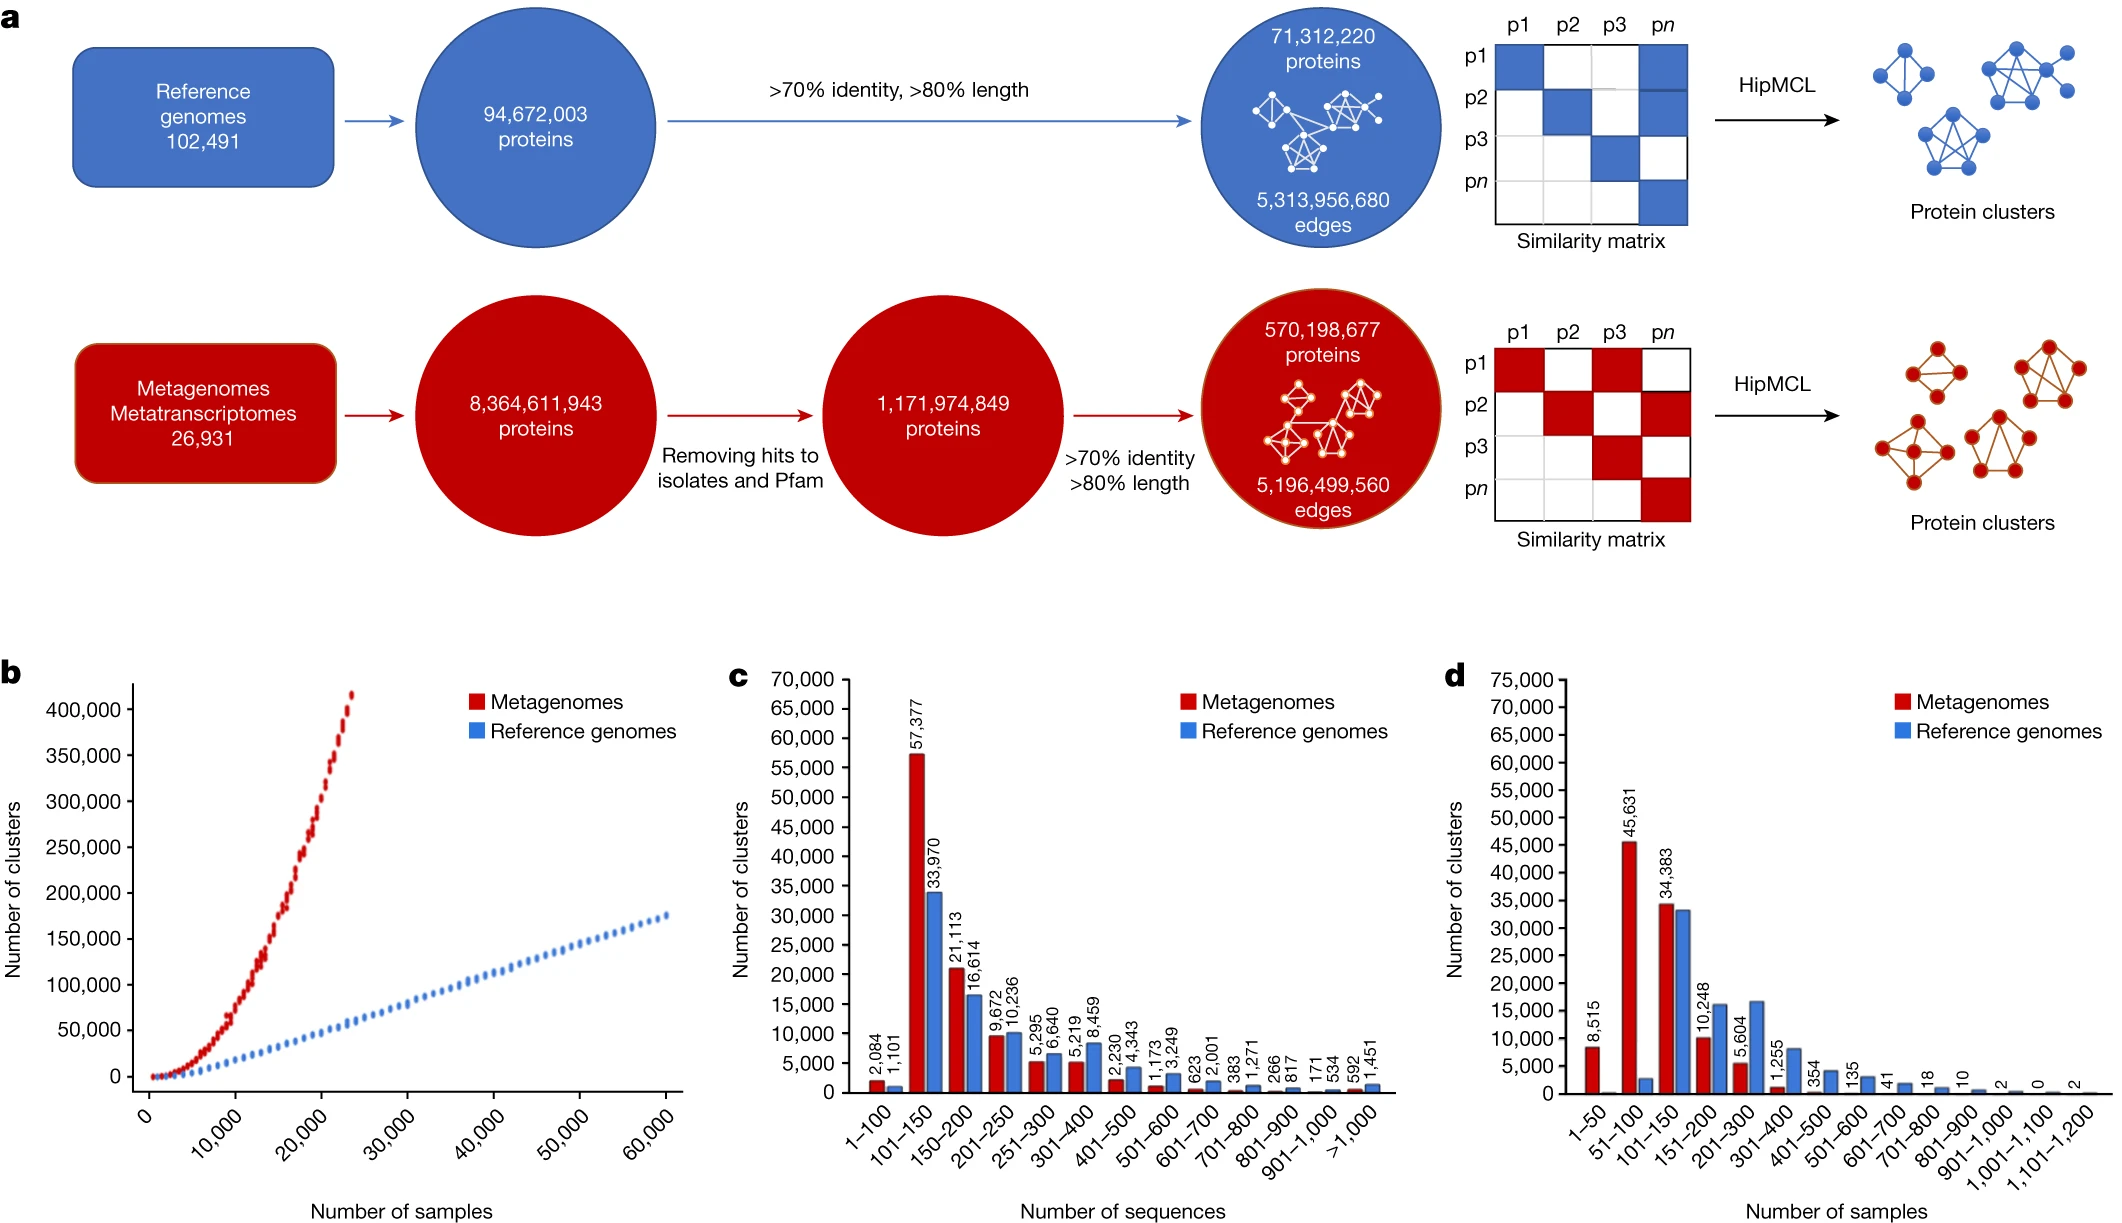
\includegraphics[width=1\linewidth]{asset/darkmatter.png}
  \caption{Overview of large-scale protein clustering from \cite{darkMatter}.
  (a) Pipeline: reference genomes (102k) and metagenomes (26k) yield billions
  of protein sequences. Pairwise similarities are filtered using thresholds of
  \(\geq\)70\% sequence identity and \(\geq\)80\% alignment coverage, producing
  sparse graphs with hundreds of millions of nodes and billions of non-trivial
  edges, which are clustered using HipMCL. (b) As new samples are added to the
  input dataset (Number of samples), this shows how many clusters appear in the
  graph cumulatively (Number of clusters). Only the clusters with at least 100
  sequences per cluster are included. (c) Cluster size distribution:
  heavy-tailed, with many small clusters and few large ones. (d)
  Cluster distribution across samples: most clusters are restricted to a small
  number of samples, while few are widely distributed. These results
  collectively highlight the scale, extreme sparsity, and structural
  heterogeneity of protein sequence similarity networks.}
  \label{fig:darkMatter}
\end{figure}
% b. Incrementally recompute pipeline after expanding the input dataset. Why rectangles instead of points for each N number of samples? Perhaps, for each sample size they re-computed the pipeline for multiple collection of N samples. The latter is not excplicitly clarified in the paper however rarefaction plots usually involve random sampling to supress bias.

From a computational perspective, large-scale sequence clustering naturally
leads to graph-based formulations. Protein sequences can be represented as
nodes in a graph, with edges encoding similarity relationships derived from
pairwise sequence alignment scores. Community detection algorithms can then be
applied to identify densely linked subgraphs corresponding to putative protein
families or functional groups. While this formulation is conceptually
straightforward, its practical implementation at scale poses significant computational challenges.

As demonstrated by \cite{ssn}, sequence similarity networks offer a scalable
and interpretable framework for visualizing relationships across large protein
superfamilies. For example, human GPCRs (G protein‑coupled receptors), a
diverse family of membrane proteins involved in cellular signaling. Overlaying
such networks with orthogonal information, such as taxonomic classification
or functional annotation, reveals functional themes and highlights outliers,
making them a powerful tool for exploratory analysis. Unlike phylogenetic
trees or multiple sequence alignments, networks can accommodate far larger
datasets while preserving both global structure and local details. An example
is shown in Fig.~\ref{fig:ssn1}.

\begin{figure}[htbp]
  \centering
  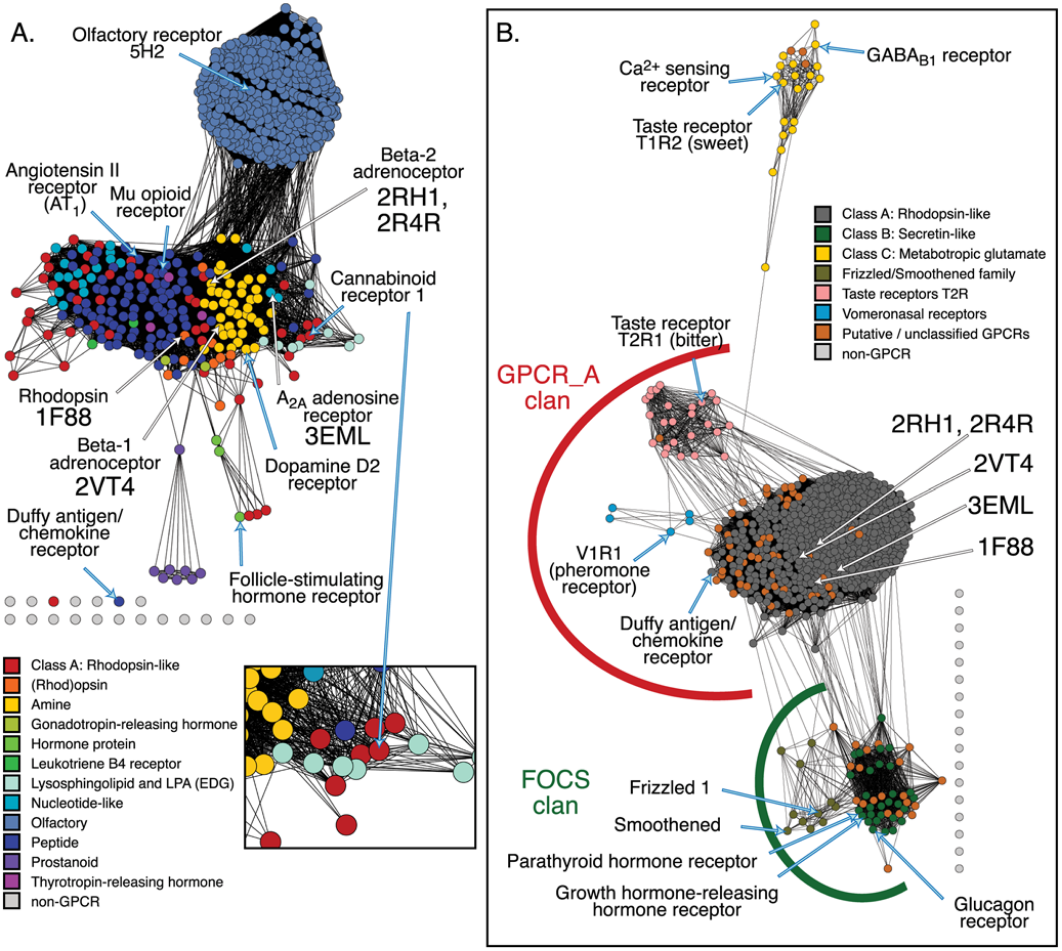
\includegraphics[width=0.9\linewidth]{asset/ssn1.png}
  \caption{Sequence similarity networks of human kinase domains from
  \cite{ssn}. Nodes represent proteins; edges indicate significant sequence
  similarity. (A) Network colored by kinase class, revealing functional
  groupings. (B) Network colored by the presence of a catalytic lysine in the
  VAIK motif, showing how orthogonal information can be overlaid to identify
  sequence features. This illustrates how sequence similarity networks can
  visualize relationships across large protein families (513 sequences) and
  overlay orthogonal information.}
  \label{fig:ssn1}
\end{figure}

\subsection*{Scope and Contribution of Current Work}

The goal of this thesis is to investigate the practical scalability of
community detection methods for protein sequence networks. Rather than
proposing new algorithms, an existing workflow is adopted and its execution is
carefully streamlined and tailored to evaluate the performance of community
detection algorithms under various configurations. Using large protein
sequence datasets derived from reference proteomes, PSSNs are constructed and
clustered using established tools, including MCL and HipMCL executed on a
single compute node.

This work is guided by three core priorities:

\begin{enumerate}
  \item \textbf{Scalability}: Establishing the practical limits of MCL and
    HipMCL on a single compute node.
  \item \textbf{Reproducibility}: Ensuring the entire workflow is
    portable, well‑documented, and executable with publicly available
    tools.
  \item \textbf{Interpretability}: Using graph‑based representations and
    alignment‑derived similarity, which provide direct biological meaning
    without black‑box embeddings.
\end{enumerate}

The primary emphasis of this study is on computational performance with limited
emphasis on the evaluation of the results. Precise biological validation of the
resulting clusters is considered outside the main scope of this work. Instead,
the focus is placed on the computational challenges that arise when applying
widely used clustering algorithms to large biological datasets on a single
compute node, and on identifying practical limitations encountered in this
environment.

By systematically documenting these observations, this thesis aims to assess
the capabilities and limitations of reproducible and interpretable community
detection applied to sparse PSSNs comprising millions of vertices representing
protein sequences. Such an assessment is intended to inform both computational
scientists developing scalable algorithms and bioinformaticians seeking to
apply these methods to large biological datasets in practical computing
environments.
